\hfill \break

\subsection*{Análisis a priori}

    Consideremos el pseudocódigo descrito en la figura \ref{PseudocodigoHuffman} para la codificacion de Huffman.

    \begin{figure}[h!]
        \centering
        \begin{verbatim}
            Huffman(C: arreglo de caracteres sin repeticion)
                n = |C|
                Q = cola_prioridad(C)
                for i=1 to i<=n do
                    x = Q.extraerMin()
                    y = Q.extraerMin()
                    z = nuevo_nodo
                    z.izq = x
                    z.der = y
                    z.frec = x.frec + y.frec
                    Q.insertar(z)
                return Q
        \end{verbatim}  
        \caption{Pseudocódigo del algoritmo de la codificacion de Huffman}
        \label{PseudocodigoHuffman}
    \end{figure}
    
    Podemos observar en la figura \ref{PseudocodigoHuffman} que el algoritmo hace uso de una cola de prioridad, llamada Q para sacar los nodos con la menor frecuencia en cada iteración. Posteriormente se crea un nuevo nodo que tiene como hoja izquierda al nodo con la menor frecuencia de los dos y como hoja derecha al que tiene una mayor frecuencia. A continuación se calcula la complejidad del algoritmo por análisis por bloque.
    
    \begin{equation*}
        \left.
            \begin{aligned}
                \left.
                    \begin{aligned}
                        \text{n = C.size} \\
                        \text{Q = colaprioridad(C)}
                    \end{aligned}
                \right\}
                \quad\Theta(1)
                \\
                \left.
                    \begin{aligned}
                        \text{for i=1 to i<=n do} \\
                        \left.
                            \begin{aligned}
                                \text{x = Q.extraerMin()} \\
                            \end{aligned}
                        \right\}
                        \quad\Theta(log(n))
                        \\
                        \left.
                            \begin{aligned}
                                \text{y = Q.extraerMin()} \\
                            \end{aligned}
                        \right\}
                        \quad\Theta(log(n))
                        \\
                        \left.
                            \begin{aligned}
                                \text{z = nuevonodo} \\
                                \text{z.izq = x} \\
                                \text{z.der = y} \\
                                \text{z.frec = x.frec + y.frec} \\
                            \end{aligned}
                        \right\}
                        \quad\Theta(log(n))
                        \\
                        \left.
                            \begin{aligned}
                                \text{Q.insertar(z)} \\
                            \end{aligned}
                        \right\}
                        \quad\Theta(log(n))
                        \\
                        \text{return Q} \\
                    \end{aligned}
                \right\}
                \quad\Theta(nlog(n))
            \end{aligned}
        \right\}
        \quad\Theta(nlog(n))
    \end{equation*}
    
    Finalmente, la complejidad del algoritmo de la codificacion de Huffman esta dado por $\Theta(nlog(n))$. Es interesante observar que usar las operaciones de extraer e insertar son las que agregan la complejidad logaritmica $\Theta(log(n))$ debido a la forma en la que insertan y extraen elementos de su heap, siendo el heap también un arbol que describe la prioridad de sus elementos. 

\subsection*{Análisis a posteriori}

    Para la generación de nuestras gráficas, se realizó un conteo del número de operaciones realizadas en el algoritmo para cada arreglo de tamaño n de caracteres sin repeticion. Se utilizaron archivos de texto que se trabajan para generar su codifcación de Huffman, su árbol asociado y su decodificacion final. Los archivos se construyeron considerando los caracteres que iban a contener quitando sus repeticiones. Por ejemplo:
    
    Teniendo como entrada un archivo que contuviera la cadena "bbbaaaccfffttat", nuestro arreglo sin repeticiones seria [b,a,c,f,t] y la n asociada sería n=5.
    
    En la figura \ref{GraficaHuffman} se presenta la gráfica generada por nuestra implementación.
    
    \begin{figure}[h!]
        \centering
        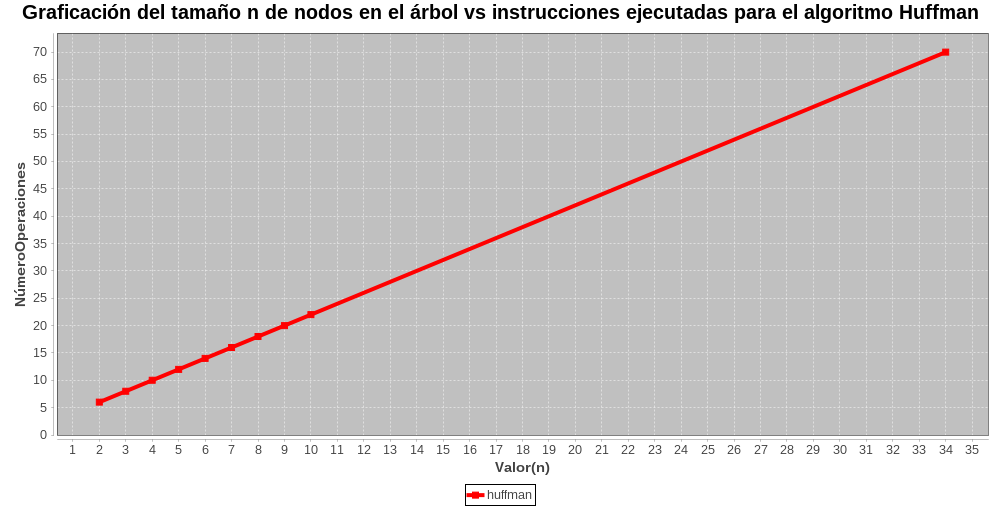
\includegraphics[width=13cm]{Huffman/graf-huffman.png}
        \caption{Representación gráfica de la complejidad temporal del algoritmo de la codificación de Huffman, mediante la evaluación del número de instrucciones realizadas.}
        \label{GraficaHuffman}
    \end{figure}
    
    Teniendo como puntos al siguiente arreglo, mostrado en la figura \ref{PuntosHuffman}:
    
    \begin{figure}[h!]
        \centering
        \begin{tabular}{c|c}
            P1( 2,6 ) & P5( 6,14 )\\
            P2( 3,8 ) & P6( 7,16 )\\
            P3( 4,10 ) & P7( 8,18 )\\
            P4( 5,12 ) & P8( 9,20 )\\
            P10( 10,22 ) & P11( 34, 70)
        \end{tabular}
        \caption{Pares obtenidos de la evaluación del algoritmo de la codificación de Huffman}
        \label{PuntosHuffman}
    \end{figure}
    
    Como se puede notar a simple vista, el algoritmo parece tener una complejidad lineal dada por $\Theta(n)$. Sin embargo, la causa de este desvio con nuestro análisis a priori fue que no se hizo una implementación propia de una cola de prioridad con sus operaciones, si no, que se utilizó la clase PriorityQueue definida por el lenguaje Java. Por lo tanto no fue posible considerar las instrucciones ejecutadas durante cada operacion de la cola de prioridad, causando que la complejidad aparente fuera lineal cuando debería ser $\Theta(nlog(n))$. A continuación en la figura , se representan los puntos en un graficador con la ecuación que los delimita $y=2x+2$ y la ecuación por la que deberían de estar acotados $y=xlog(x)$.
    
    \begin{figure}[h!]
        \centering
        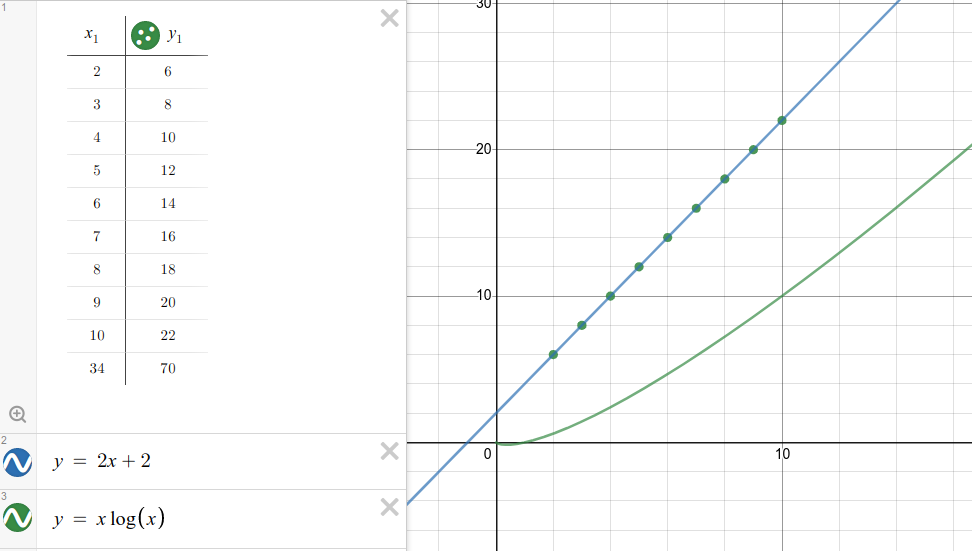
\includegraphics[width=13cm]{Huffman/graf-desm-huffman.png}
        \caption{Representación gráfica de la complejidad temporal del algoritmo de la codificación de Huffman, comparado con la ecuacion que los delimita en color azul $y=2x+2$ y la ecuación por la que deberian de estar acotados $y=xlog(x)$}
        \label{GraficaHuffman}
    \end{figure}
    \newpage
    
\subsection*{Proceso de compresión y descompresión}
    
    Para comprimir nuestro archivo de entrada sustituimos cada caracter por su representación de la conficación de Huffman que se guarda en un diccionario, y se forma una nueva cadena con una representación binaria de la salida comprimida. \\
    
    Para descomprimir una cadena que esta en su representación de Huffman, necesitamos el arbol que contiene su representación. Se recorre el arbol y si se alcanza una de las hojas, se extrae el caracter que representa y se guarda en un string que tendrá como salida a la cadena decodificada. \\
    
    La tasa de compresión se calcula considerando que la cadena de entrada original esta codificada en utf-8, por lo que cada caracter representa un byte, es decir, 8 bits. En nuestra salida codificada, cada caracter representa un bit. Finalmente, mediante una regla de 3, siendo el 100\% el numero de bits de la cadena original, calculamos la tasa de compresión.
    
    \subsubsection{Ejemplo 1}
        \begin{itemize}
            \item \textbf{Texto de origen} \\
            Era de noche. En la vasta sala silenciosa, tenuemente alumbrada por unas luces ocultas en los muros transparentes, los cuatro terrestres, sentados alrededor de
una mesa de madera conversaban en voz baja, con los rostros juntos y pálidos.
Hombres y mujeres yacían desordenadamente por el suelo. En los rincones
oscuros había leves estremecimientos: hombres o mujeres solitarios que movían
las manos. Cada media hora uno de los terrestres intentaba abrir la puerta de
plata.
-No hay nada que hacer. Estamos encerrados.
-¿Creen realmente que somos locos, capitán?
-No hay duda. Por eso no se entusiasrnaron al vernos. Se limitaron a tolerar lo que
entre ellos debe de ser un estado frecuente de psicosis. -Señaló las formas
oscuras que yacían alrededor.-Paranoicos todos. ¡Qué bienvenida! -Una llamita se
alzó y murió en los ojos del capitán.-Por un momento creí que nos recibían como
merecíamos. Gritos, cantos y discursos. Todo estuvo muy bien, ¿no es cierto?
Mientras duró. 
            \item \textbf{Compresión} \\
                \begin{figure}[h!]
                    \centering
                    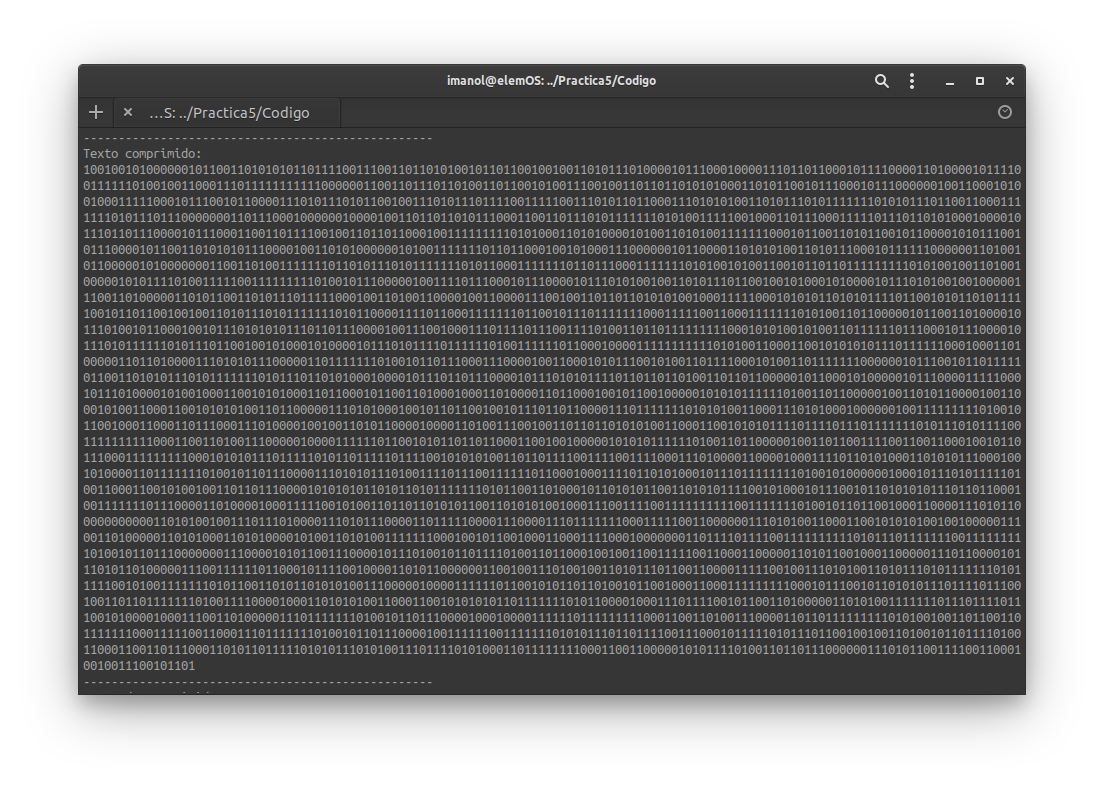
\includegraphics[width=17cm]{Huffman/ejemplos/ejemplo1/ej1-comp.png}
                \end{figure}
                \newpage
            \item \textbf{Tasa de compresión:} 54.296875\% \\
            \item \textbf{Descompresión} \\
                \begin{figure}[h!]
                    \centering
                    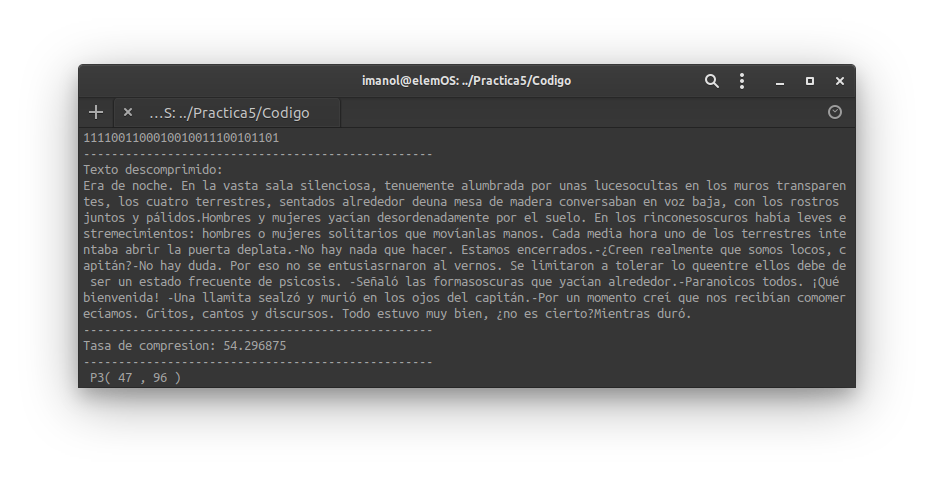
\includegraphics[width=17cm]{Huffman/ejemplos/ejemplo1/ej1-decode.png}
                \end{figure}
                \newpage
            \item \textbf{Codificación asignada} \\
                \begin{figure}[h!]
                    \centering
                    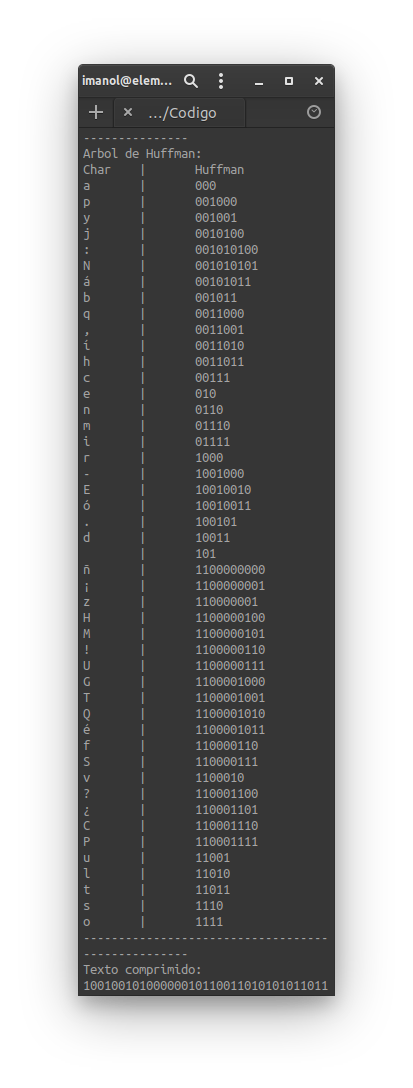
\includegraphics[scale=.5]{Huffman/ejemplos/ejemplo1/ej1-reph.png}
                \end{figure}
                \newpage
        \end{itemize}
    \subsubsection{Ejemplo 2}
        \begin{itemize}
            \item \textbf{Texto de origen} \\
            Las llamas azules brotaban alrededor de los terrestres, brillaban un momento, y se
desvanecían. Unos diablillos de arena roja corrían entre los dientes de los
hombres dormidos. Las mujeres se transformaban en serpientes aceitosas. Había
un olor de reptiles y bestias. 
            \item \textbf{Compresión} \\
                \begin{figure}[h!]
                    \centering
                    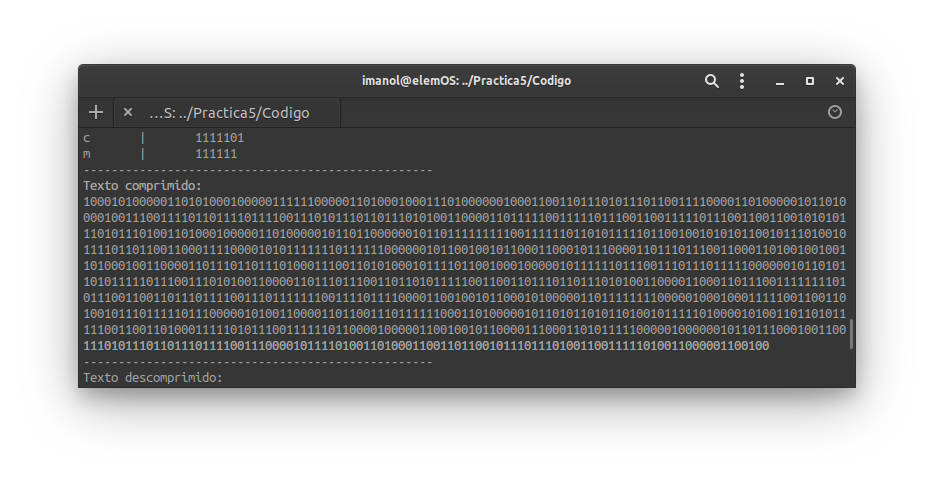
\includegraphics[width=17cm]{Huffman/ejemplos/ejemplo2/ej2-comp.png}
                \end{figure}
                \newpage
            \item \textbf{Tasa de compresión:} 51.089016\% \\
            \item \textbf{Descompresión} \\
                \begin{figure}[h!]
                    \centering
                    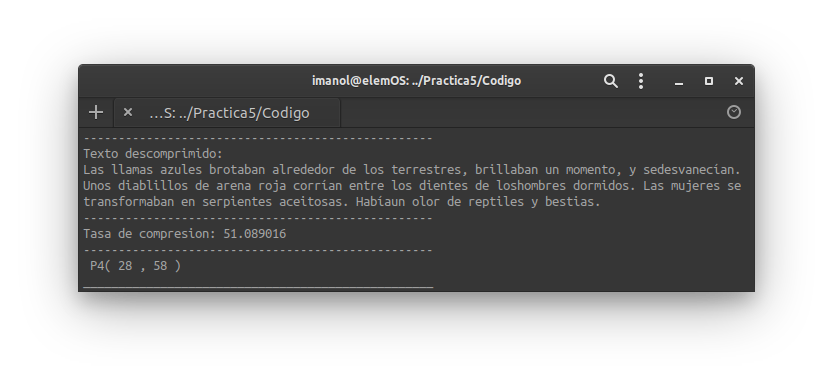
\includegraphics[width=17cm]{Huffman/ejemplos/ejemplo2/ej2-decode.png}
                \end{figure}
                \newpage
            \item \textbf{Codificación asignada} \\
                \begin{figure}[h!]
                    \centering
                    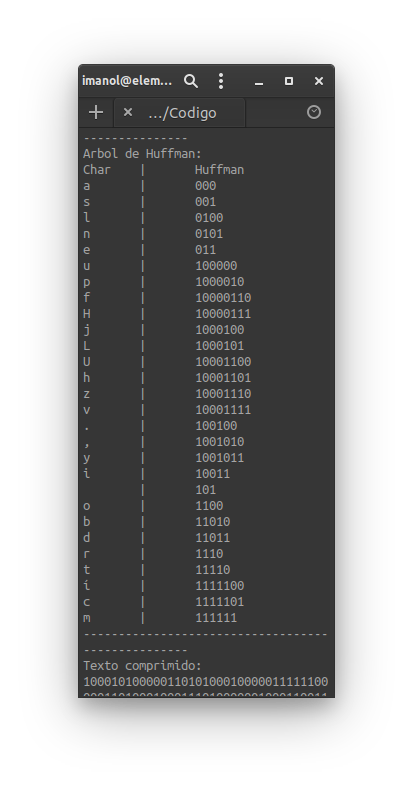
\includegraphics[scale=.5]{Huffman/ejemplos/ejemplo2/ej2-reph.png}
                \end{figure}
                \newpage
        \end{itemize}
    \subsubsection{Ejemplo 3}
        \begin{itemize}
            \item \textbf{Texto de origen} \\
            Qué demencia más hermosa. Metal, caucho, gravitadores, comida, ropa,
combustible, armas, escaleras, tuercas, cucharas. He comprobado que en su nave
hay diez mil artículos distintos. Nunca había visto tal complejidad. Hay hasta
sombras debajo de las literas y debajo de todo. ¡Qué poder de concentración! Y
todo, no importan cuándo o cómo se pruebe, tiene olor, solidez, gusto, sonido.
Permítame que lo abrace.-El psiquiatra abrazó al capitán.- Consignaré todo esto
en lo que será mi mejor monografia. El mes que viene hablaré en la Academia
Marciana. Mírese. Ha cambiado usted hasta el color de sus ojos, del amarillo al
azul, y la tez de morena a sonrosada. ¡Y su ropa, y sus manos de cinco dedos en
vez de seis! ¡Metamorfosis biológica a través del desequilibrio psicológico! Y sus
tres amigos... 
            \item \textbf{Compresión} \\
                \begin{figure}[h!]
                    \centering
                    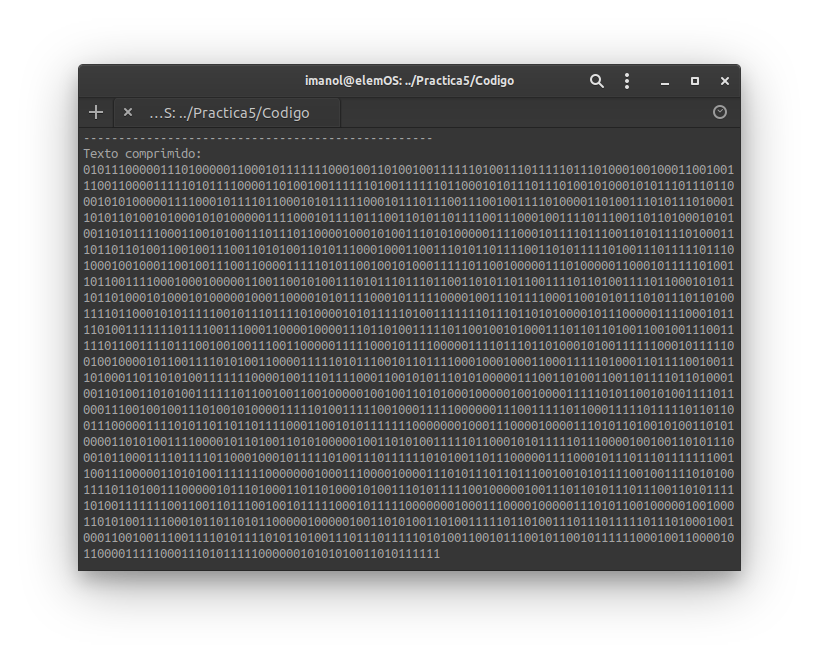
\includegraphics[width=17cm]{Huffman/ejemplos/ejemplo3/ej3-comp.png}
                \end{figure}
                \newpage
            \item \textbf{Tasa de compresión:} 56.04378\% \\
            \item \textbf{Descompresión} \\
                \begin{figure}[h!]
                    \centering
                    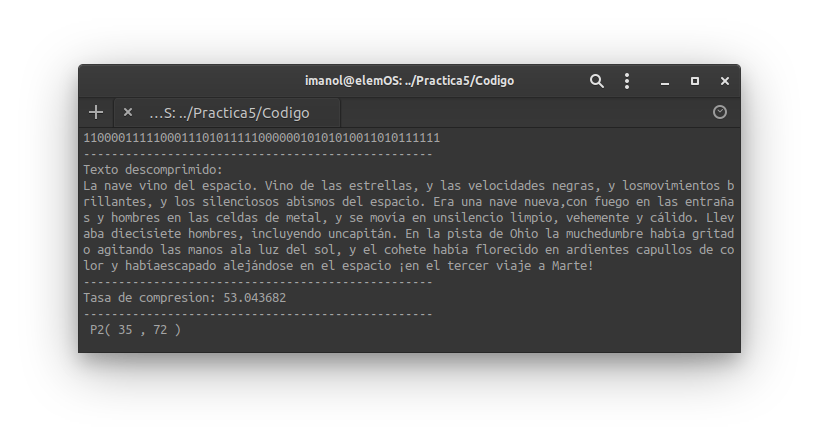
\includegraphics[width=17cm]{Huffman/ejemplos/ejemplo3/ej3-decode.png}
                \end{figure}
                \newpage
            \item \textbf{Codificación asignada} \\
                \begin{figure}[h!]
                    \centering
                    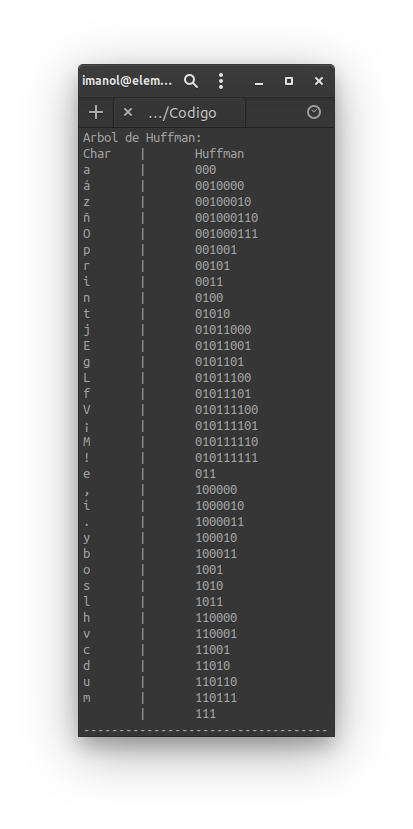
\includegraphics[scale=.5]{Huffman/ejemplos/ejemplo3/ej3-reph.png}
                \end{figure}
                \newpage
        \end{itemize}
    \subsubsection{Ejemplo 4}
        \begin{itemize}
            \item \textbf{Texto de origen} \\
            Quería ir a Marte en el cohete. Bajó a la pista en las primeras horas de la mañana
y a través de los alambres les dijo a gritos a los hombres uniformados que quería
ir a Marte. Les dijo que pagaba impuestos, que se llamaba Pritchard y que tenía el
derecho de ir a Marte. ¿No había nacido allí mismo en Ohio? ¿No era un buen
ciudadano? Entonces, ¿por qué no podía ir a Marte? Los amenazó con los puños
y les dijo que quería irse de la Tierra; todas las gentes con sentido común querían
irse de la Tierra. Antes que pasaran dos años iba a estallar una gran guerra
atómica, y él no quería estar en la Tierra en ese entonces. Él y otros miles como
él, todos los que tuvieran un poco de sentido común, se irían a Marte. Ya lo iban a 
32
ver. Escaparían de las guerras, la censura, el estatismo, el servicio militar, el
control gubernamental de esto o aquello, del arte y de la ciencia. ¡Que se
quedaran otros! Les ofrecía la mano derecha, el corazón, la cabeza, por la
oportunidad de ir a Marte. ¿Qué había que hacer, qué había que firmar, a quién
había que conocer para embarcar en un cohete?

Los hombres de uniforme se rieron de él a través de los alambres. No quería ir a
Marte, le dijeron. ¿No sabía que las dos primeras expediciones habían fracasado y
que probablemente todos sus hombres habían muerto?
            \item \textbf{Compresión} \\
                \begin{figure}[h!]
                    \centering
                    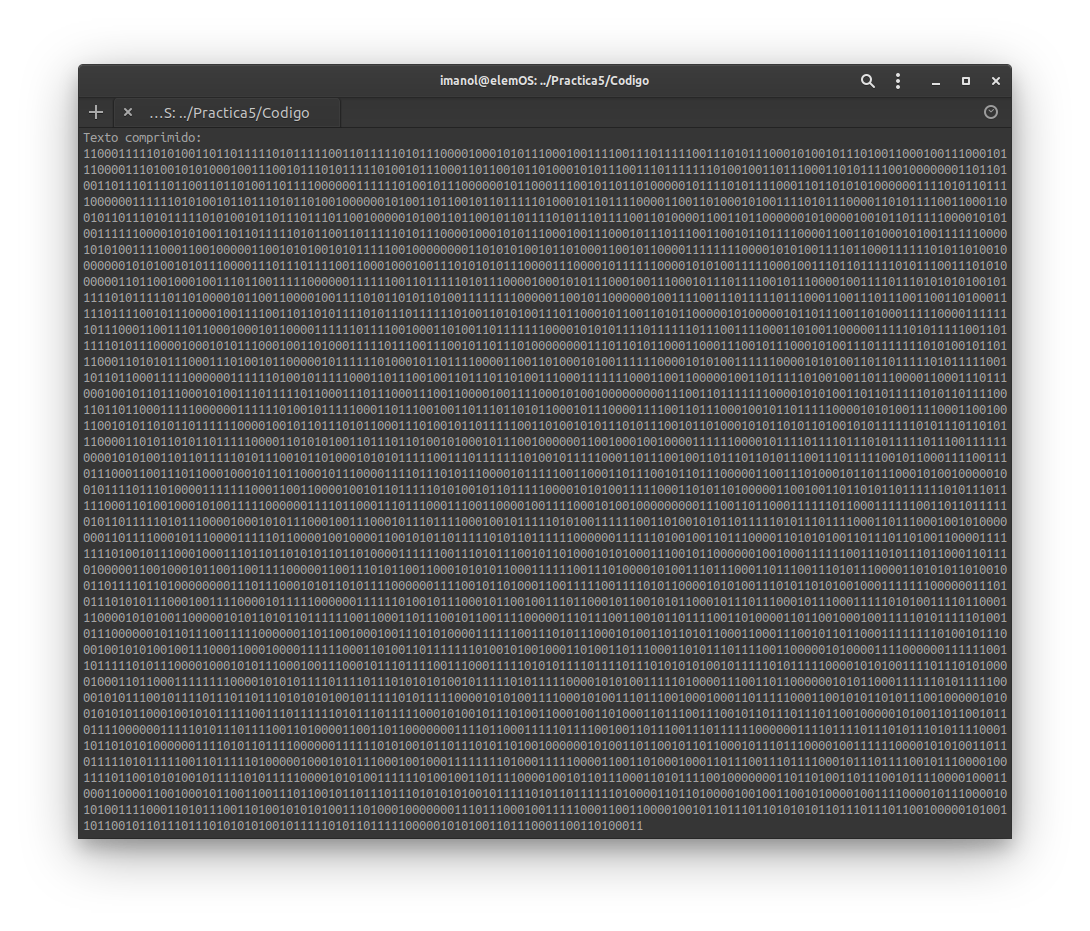
\includegraphics[width=17cm]{Huffman/ejemplos/ejemplo4/ej4-comp.png}
                \end{figure}
                \newpage
            \item \textbf{Tasa de compresión:} 54.70817\% \\
            \item \textbf{Descompresión} \\
                \begin{figure}[h!]
                    \centering
                    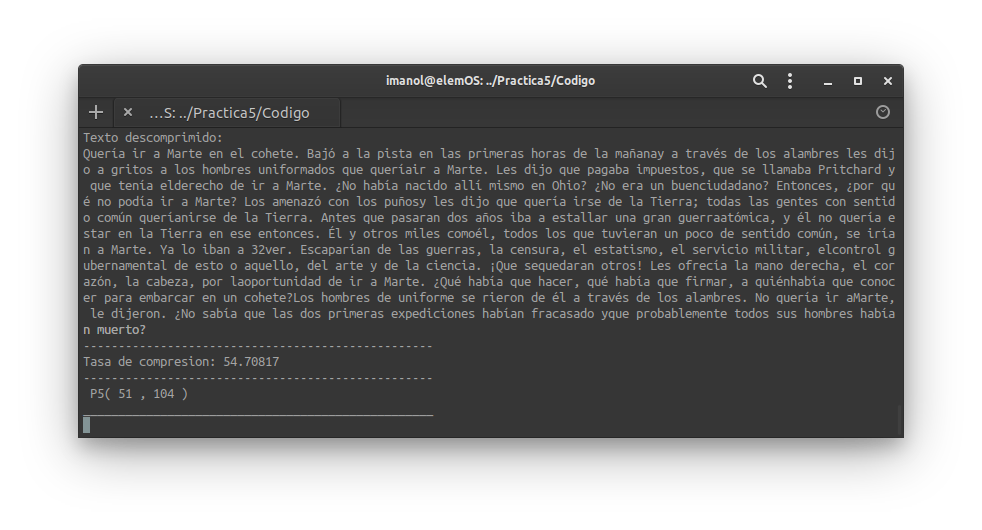
\includegraphics[width=17cm]{Huffman/ejemplos/ejemplo4/ej4-decode.png}
                \end{figure}
                \newpage
            \item \textbf{Codificación asignada} \\
                \begin{figure}[h!]
                    \centering
                    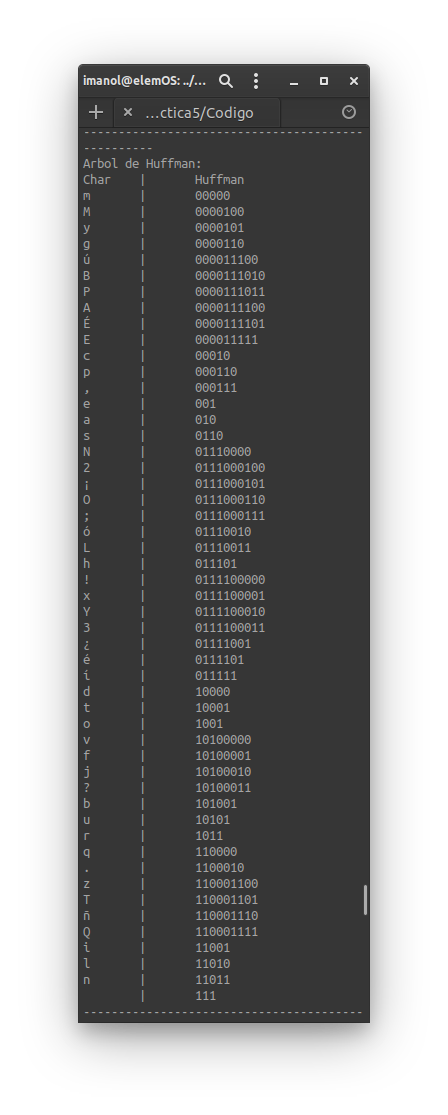
\includegraphics[scale=.5]{Huffman/ejemplos/ejemplo4/ej4-reph.png}
                \end{figure}
                \newpage
        \end{itemize}
    \subsubsection{Ejemplo 5}
        \begin{itemize}
            \item \textbf{Texto de origen} \\
            La nave vino del espacio. Vino de las estrellas, y las velocidades negras, y los
movimientos brillantes, y los silenciosos abismos del espacio. Era una nave nueva,
con fuego en las entrañas y hombres en las celdas de metal, y se movía en un
silencio limpio, vehemente y cálido. Llevaba diecisiete hombres, incluyendo un
capitán. En la pista de Ohio la muchedumbre había gritado agitando las manos a
la luz del sol, y el cohete había florecido en ardientes capullos de color y había
escapado alejándose en el espacio ¡en el tercer viaje a Marte! 
            \item \textbf{Compresión} \\
                \begin{figure}[h!]
                    \centering
                    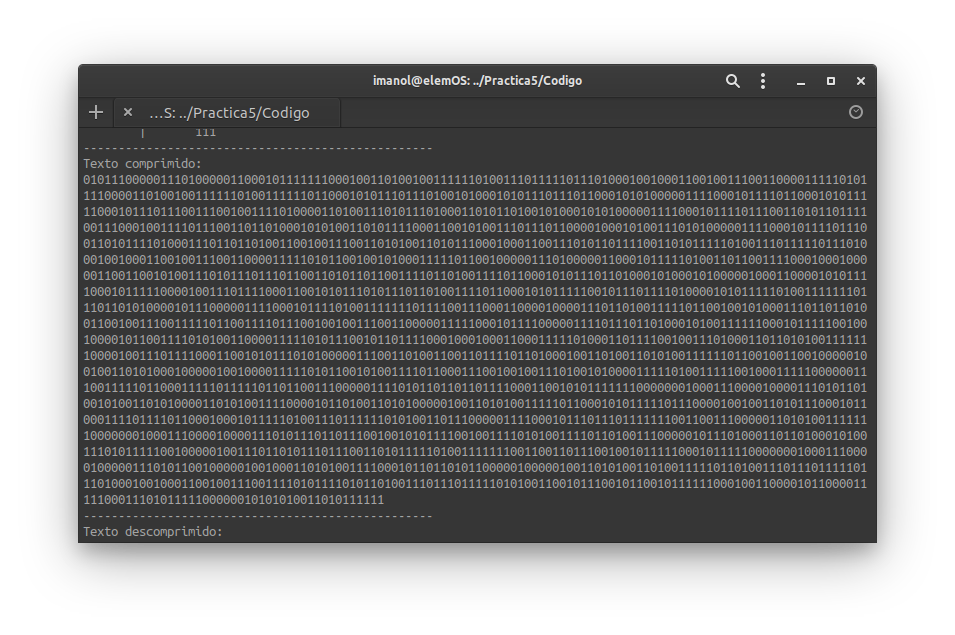
\includegraphics[width=17cm]{Huffman/ejemplos/ejemplo5/ej5-comp.png}
                \end{figure}
                \newpage
            \item \textbf{Tasa de compresión:} 53.043682\% \\
            \item \textbf{Descompresión} \\
                \begin{figure}[h!]
                    \centering
                    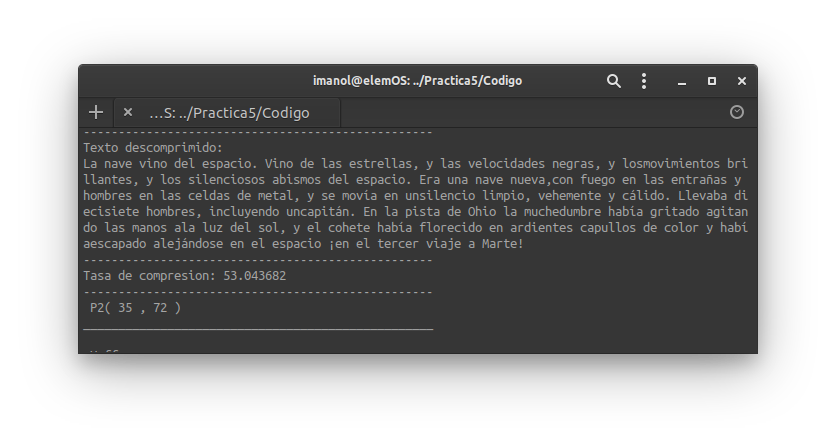
\includegraphics[width=17cm]{Huffman/ejemplos/ejemplo5/ej5-decode.png}
                \end{figure}
                \newpage
            \item \textbf{Codificación asignada} \\
                \begin{figure}[h!]
                    \centering
                    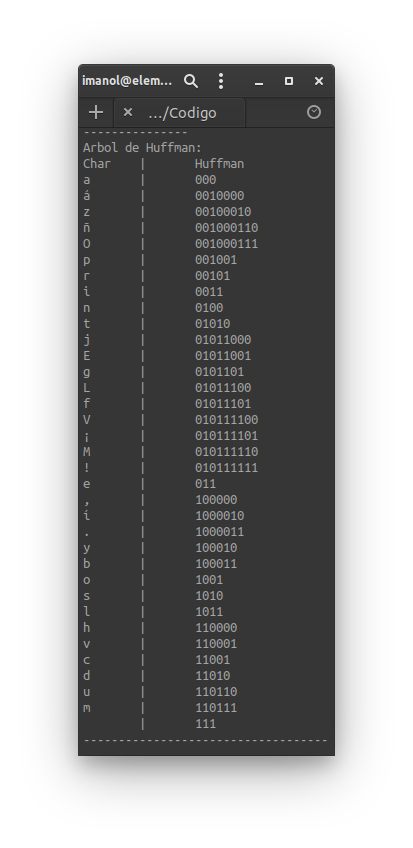
\includegraphics[scale=.5]{Huffman/ejemplos/ejemplo5/ej5-reph.png}
                \end{figure}
                \newpage
        \end{itemize}